\documentclass{article} % For LaTeX2e
% We will use NIPS submission format
\usepackage{nips13submit_e,times}
% for hyperlinks
\usepackage{hyperref}
\usepackage{url}
% For figures
\usepackage{graphicx} 
\usepackage{subfigure} 
% math packages
\usepackage{amsmath}
\usepackage{amsfonts}
\usepackage{amsopn}
\usepackage{ifthen}
\usepackage{natbib}

% ///////////////////////////////////////////////////////////
% //////////////////// Comments from Emti ///////////////////
% ///////////////////////////////////////////////////////////
%
%- Your report should not be longer than 6 pages!
%- Your report should include the details of your work, e.g. you can include the following 
%points:
%  - What feature transformation or data cleaning did you try? And why?
%  - What methods you applied? Why?
%  - What worked and what did not? Why do you think are the reasons behind that?
%  - Why did you choose the method that you choose?
%- You should include complete details about each algorithm you tried, e.g. what lambda values 
%you tried for Ridge regression? What feature transformation you tried? How many folds did you 
%use for cross-validation? etc.
%- You should include figures or tables supporting your text and your conclusions.
%- Make sure that the captions are included in the figure/tables. A caption should clearly 
%describe the content of its corresponding figure/table.
%- Please label your figures and make sure that the labels and legends are large enough to be 
%read clearly.
%- Make sure that the tick marks and labels are large enough to be clearly read.
%- Your sentences in the report should be clear, concise, and direct.
%- You should clearly state your conclusions.
%- You will loose marks if you did not do things mentioned above.
%- You will loose marks if your written text is vague and not understandable!
%
% ///////////////////////////////////////////////////////////
% ////////////////////// Report outline /////////////////////
% ///////////////////////////////////////////////////////////
%
%Abstract
%- describe the problem, the proposed solution with a little justification, and the results (4-5 sentences)
%
%1. Introdction
%- general introduction about the project and the learning outcomes (4-5 sentences)
%
%
%2. Regression
%- a short discussion about regression (2-3 sentences)
%
%2.1. Data description
%- description of the train and test data for regression
%
%2.2. Data visualization and cleaning
%- outlier detection and removal (add a histogram of y to show the outliers)
%- (add Andrii's graph which shows the correlation between the input and output variables) - table with the e.g. 5 most significant (most correlated) features
%- data separation (X_30 > -10.5 and X_30 <= -10.5)
%
%2.3. Feature transformations
%- methodology (how do we normalize)
%- choice of different basis functions and how do they influence our predictions for left/right 
%dataset (x^3 for the right dataset) - add a figure/table to compare it with no transformation
%- why PCA is not a good choice (graph of eigenvalues)
%
%2.4. Experimental results
%- choose a baseline
%- (procedure and results obtained by using gradient desc. (also, why is it not good/sufficient))
%- procedure and results obtained by using least squares (also, why is it not good/sufficient)
%- procedure and results obtained by using ridge regression (also, why is it not good/sufficient)
%- (add a fancy regression method)
%- learning curve - plot how the train/test errors change (mean + variance with multiple seeds) as we assign more data to training (keep the test data at e.g. 20%)
%- Fig: train/test errors for different train data proportions (least squares + ridge regression)
%- Fig: train/test errors for different train lambda (ridge regression)
%- fitting one linear model for both datasets (left and right) could work but will be more complicated
%
%
%3. Classification
%- a short discussion about classification (2-3 sentences)
%
%3.1. Data description
%- description (N, D, cathegorical data) of the train and test data for classification
%
%3.2. Data visualization and cleaning
%- outlier detection and removal (add a histogram of y to show the outliers)
%- (add Andrii's graph which shows the correlation between the input and output variables)
%
%3.3. Feature transformations
%- choice of different basis functions and how they influence our predictions - a table
%- (why PCA is not a good choice + graph of eigenvalues)
%
%3.4. Experimental results
%- choose a baseline
%- (procedure and results obtained by using linear regression (why is it not good))
%- procedure and results obtained by using logistic regression (why is it not good/sufficient)
%- procedure and results obtained by using penLogistic regression (why is it not good/sufficient)
%- (add a fancy classification method)
%- learning curve - plot how the train/test errors change (mean + variance with multiple seeds) 
%as we assign more data to training (keep the test data at e.g. 20%)
%- Fig: train/test errors for different train data proportions (least squares + ridge regression)
%- Fig: train/test errors for different train lambda (ridge regression)
%
%
%4. Conclusion
%- paragraph about the conclusions from regression (4-5 sentences)
%- paragraph about the conclusions from classification (4-5 sentences)
%- state the limitations of these approaches and give directions for future work

\title{Project-I by Group LasVegas}

\author{
Igor Kulev \\
EPFL \And
Andrii Maksai \\
EPFL \And
Marjan Shahpaski \\
EPFL \\\\
\texttt{\{igor.kulev, andrii.maksai, marjan.shahpaski\}@epfl.ch}\\
}

% The \author macro works with any number of authors. There are two commands
% used to separate the names and addresses of multiple authors: \And and \AND.
%
% Using \And between authors leaves it to \LaTeX{} to determine where to break
% the lines. Using \AND forces a linebreak at that point. So, if \LaTeX{}
% puts 3 of 4 authors names on the first line, and the last on the second
% line, try using \AND instead of \And before the third author name.

\nipsfinalcopy 

\begin{document}

\maketitle

\begin{abstract}
This report provides a summary of our work done for the first project of the PCML course. 
The project consists of solving two problems: a regression and a classification problem. 
For the regression dataset, we have noticed two separate clusters of data. 
Therefore, we separated the data in two parts, and have applied different linear models to each part. 
To the classification dataset, we applied logistic regression and penalized
logistic regression.
In addition, we have investigated a few feature transformations which provided some additional improvements.
\end{abstract}

\section{Introduction}

The first project of the Pattern Classification and Machine Learning course focuses on 
applying linear models to regression and classification problems. 
The ultimate goal is to train a model which will be able to produce accurate response predictions 
to unseen input data. The unseen data is assumed to be produced by the same source(s) as the training data. 
The tasks involved in solving these problems are preprocessing the data, 
training linear models for the corresponding regression/classification tasks, 
and applying appropriate feature transformations to the input variables.

%The algorithms which we use for regression are least squares and ridge
% regression.
%For classification, we have implemented logistic regression and penalized
% logistic regression.

\section{Regression}

Regression models try to establish the relationships between the input and the output variables(s). 
It is used for predicting future outcomes for new (unobserved) data, or for interpreting 
the underlying connection(s) between the input and the output variables. 
In this project we will use linear regression models, which assume a linear relation between the 
inputs and the outputs. 
We will also use non-linear feature transforms, however the regression parameters will remain linear.

\subsection{Data Description}

The training data for regression consists of $N_{tr}=1400$ input and output data samples. 
Each input sample is a vector $\mathbf{x}_n$ with dimensionality $D=38$. 
All input samples are stored together in the matrix $\mathbf{X}_{tr}$. 
The output variables are scalar, and they are stored in the vector $\mathbf{y}_{tr}$. 
Each input vector $\mathbf{x}_n$ contains 30 real valued variables and 8 categorical variables. 
From the categorical variables, 1 is binary (variable 37), 3 have three 
categories (variables 31, 33 and 34), and 4 have four categories (variables 32, 35, 36 and 38).

The test dataset $\mathbf{X}_{te}$ consists of $N_{te}=600$ samples.
The goal is to train a regression model by using the training data $\mathbf{X}_{tr}$, and 
then use it to produce predictions $\mathbf{\hat{y}}_{te}$ for the unknown
output variables $\mathbf{y}_{te}$. 
Test error for unseen data for our model is reported in the form of RMSE.

\subsection{Data visualization and cleaning}

\begin{figure}[!t]
	\center
	\subfigure[Correlation of the 30th feature with the response. We assume that
	the data was generated by two sources. The data points encircled in red are the outliers produced by our initial classification.] {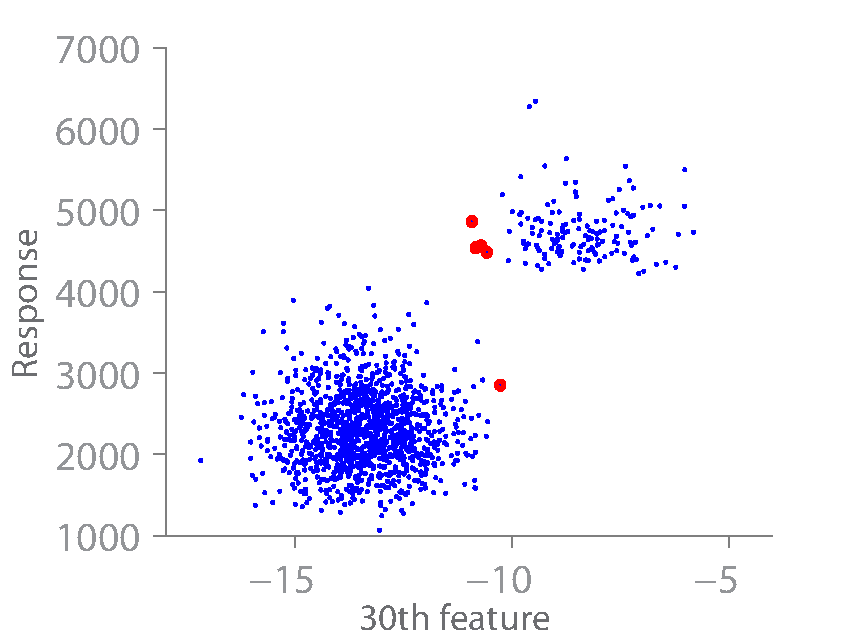
\includegraphics[trim=0mm 0mm 12mm 6mm, clip=true, width=.475\columnwidth]{figures/RegressionFeature30.pdf}
		\label{fig:RegressionFeature30}}
	\hfill
	% trim option's parameter order: left bottom right top
	\subfigure[Strong correlation between the 26th feature and the response for the points from the "right" cluster. The single outlier is encircled in red.]
		{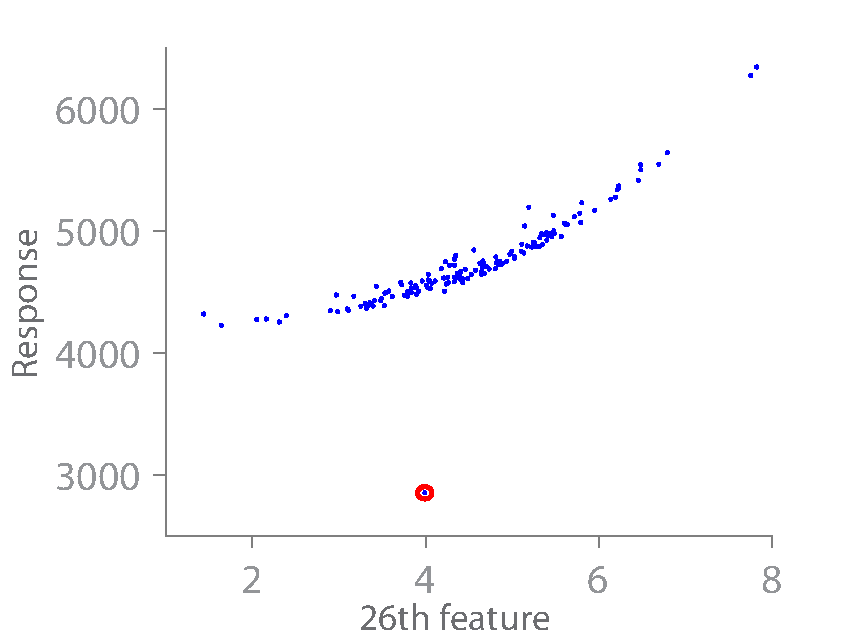
\includegraphics[trim=0mm 0mm 12mm 6mm, clip=true, width=.475\columnwidth]{figures/RegressionFeature26Right.pdf}
		\label{fig:RegressionFeature26Right}}
	\caption{Input-output data correlation and outlier visualization.}
\end{figure}

 While doing the exploratory data analysis, we found out that out of 30
 continious predictors 29 appear to have a Gaussian-like distribution of their
 values and have correlation of about 0.2-0.4 with the response, 8 categorical
 variables have correlation between -0.1 and 0.1, and 30th feature has a high
 correlation of about 0.8, and has a distribution that looks like a combination
 of two Gaussian distributions.
  Figure \ref{fig:RegressionFeature30} shows the
 response as a function of the 30th feature.
 From the figure we can see two clusters of points, and that the 30th feature
 provides a very clear separation between them.
  By visual inspection, we have concluded that the value of -10.5 of the 30th
  feature provides the cleanest separation between the "left" from the "right" clusters.

After we separate the "left" and the "right" clusters, we eliminate the outliers. 
The best separation boundary at -10.5 for the 30th feature misclassifies five data samples. 
They are shown encircled in red on Figure \ref{fig:RegressionFeature30}. 
The encircled samples which have a response between 4500 and 5000 are classified in the "left" dataset 
and represent the only outliers. In particular, we found out that for first 29
features number of points outside of 3, 4 and 5 standard deviations from the
mean is not more than is expected to be for normal distribution, therefore we
did not remove them as outliers.

On Figure \ref{fig:RegressionFeature26Right} we show the response vs. the 26th feature 
for the data samples in the "right" cluster. 
We see a very clear pattern followed by all data samples except the one encircled with red, 
which is a result from the misclassification. 
We manually remove the outliers from both clusters.

We normalize the input variables to have zero mean 
and unit variance for all training data, or for each data cluster separately,
 depending on the algorithm used (explained in the following subsection). 
 For the categorical variables which have more that 2 categories we have used dummy encoding. 
 Due to this encoding, the final number of input variables has increased from 32 to 50.

\subsection{Results}

\begin{figure}[t!]
	\center
	% trim option's parameter order: left bottom right top
	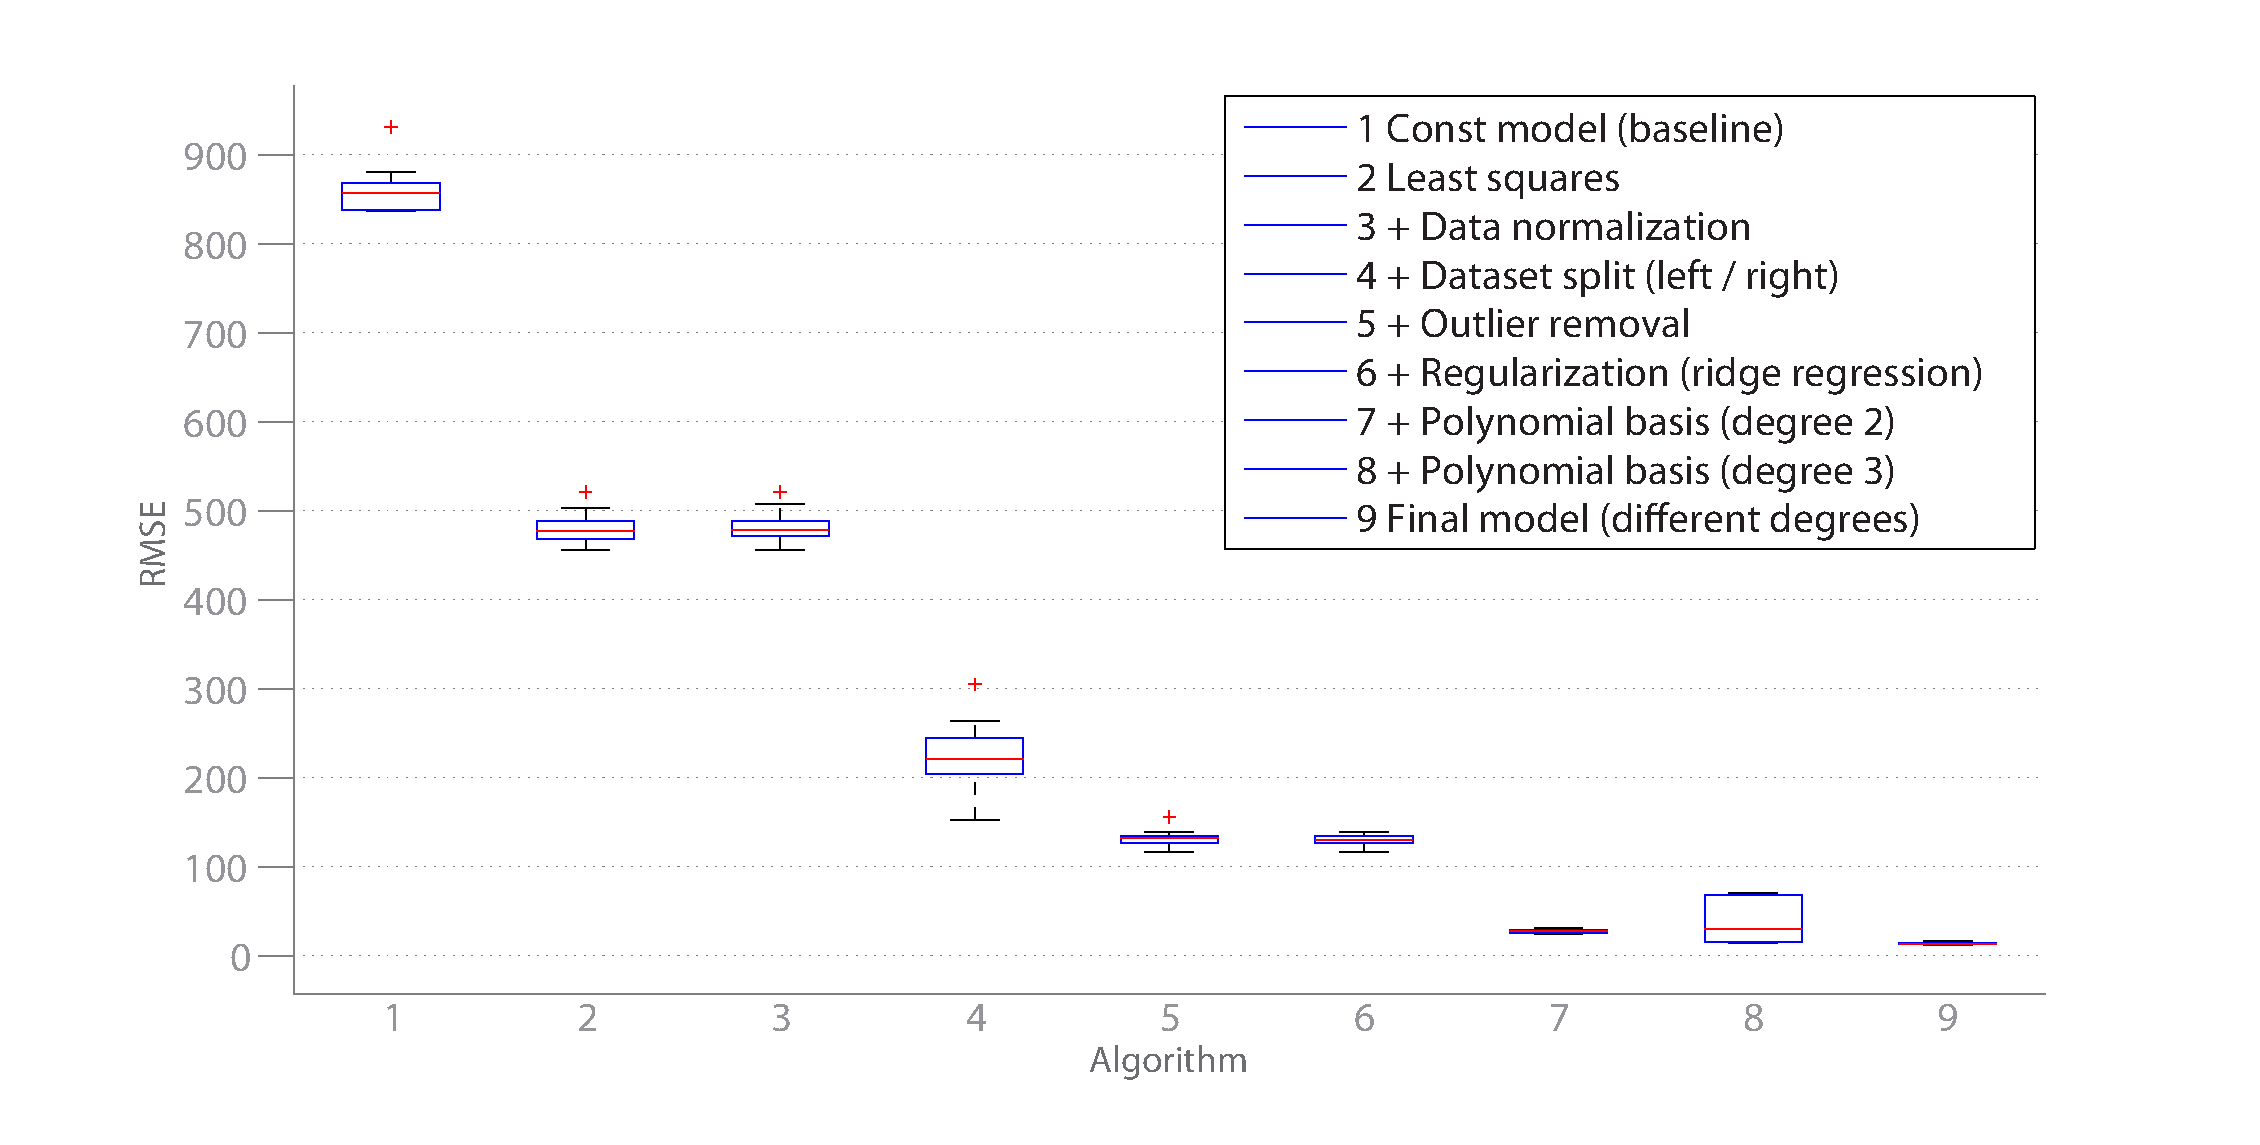
\includegraphics[trim=23mm 10mm 35mm 10mm, clip=true, width=1\columnwidth]{figures/RegressionHist3.pdf}
	\caption{The box plots show an overview of the mean and standard deviation of the different regression methods and feature transformations which we have tried. Our model of choice is \#9.}
	\label{fig:RegressionHist}
\end{figure}

\subsubsection{Evaluation procedure}

For finding the best solution for the regression task we have tried several
variations of linear regression methods with different feature
transformations.
Figure \ref{fig:RegressionHist} gives an overview of the test error RMSE performance of the different methods. 
For producing the test RMSE, we have divided our input training dataset $\mathbf{X}_{tr}$ in two parts, 
training and testing with 80\%-20\% ratio, respectively. 
The model parameters were computed by using only the training set, 
and the test RMSE was computed on the test set of data.
 Where required, the additional parameters of the models (e.g. polynomial basis degree, lambda) 
 were computed by applying a 10 fold cross validation only on the training set. 
 The computation of the test RMSE was repeated 10 times, and with 
 each trial we selected the train and test sets by random permutations, and by
  keeping the data ratio constant. 
  We will justify the choice of 80\%-20\% train-test split ratio in the following text,
   by plotting the learning curve (Figure \ref{fig:RegressionLearningCurve}).

\subsubsection{Algorithms comparison}

The first algorithm in Figure \ref{fig:RegressionHist} is the baseline; 
it is just the mean of the output variable, and it does not depend on the input variables. 
For the second model, we apply least squares, and gradually increase its complexity by adding 
different features. 
From the sixth model, we use ridge regression, 
and, together with some data manipulation and feature transformations, 
we select it as the best algorithm for making predictions for our dataset.

Least squares easily outperforms the baseline algorithm. 
This is expected, since we previously observed that the input features are correlated with the output. 
We use all 50 input features in the model. 
As it can be seen from algorithm 3, normalizing the input variables does not provide an improvement 
for this dataset. However, when we split our data according to the 30th feature, as explained in the 
previous subsection, we experience a great improvement.
 In this case, we compute different model coefficients for the "left" and the "right" cluster.
  As a next step, we remove the outliers before training the model. 
  This leads to an unexpectedly large increase in the performance of the model, 
  although there are 4 outliers out of 1255 data points in the "left" and 1 outlier out of 145 
  data points in the "right" split. %($\approx$0.4\%) and ($\approx$0.8\%)

When applying least squares we have noticed that we have some correlated
predictors. To overcome the problem of ill-conditioning we have used ridge
regression.


We selected the optimal lambda for ridge regression from the range [10$^{-5}$, 10$^2$] 
by testing 100 values in between, and choosing the lambda which minimizes validation RMSE, 
by employing 10 fold cross validation. We did not penalize the intercept $\beta_0$, which had 
values greater than 1000 for our dataset. The optimal lambda for both data splits 
are $\lambda_L$=5.4e-01 and $\lambda_R$=4.7e-02. 
Resorting to ridge regression only slightly improved the test RMSE and its variance, 
however, it solved the problem of correlated predictors.

%We applied least-squares and ridge regression to this dataset. Since the matrix is ill-conditioned, least-squares is not suitable. Therefore, we report results obtained with ridge regression alone. Note that the improvements using ridge regression were modest and not much lower than that of linear regression, however we do not expect least-squares to work well when there is a lot of testing data available. 

%Figure \ref{fig:ridgeCurve} shows the results obtained with ridge regression when we use $50\%$ of the data as test data and rest as training data. We varied the value of $\lambda$ from $10^{-4}$ to $10^3$, choosing total 500 points in between. We can see that there is a small improvement obtained for some values of $\lambda$.

%We did experiments to plot a learning curve for this data (see Andrew Ng's notes about the learning curve). We held out 20\% of data as test data and rest as training data. We chose to slowly increase the proportion of data used for training. For each proportion of the training data, we repeated the experiment 30 times to compute the distribution of error. We fit ridge regression to each sampled training set and test it on the same $20\%$ test data. We varied the value of $\lambda$ from $10^{-4}$ to $10^3$, choosing total 500 points in between.

%This gives us the learning curve shown in Fig. \ref{fig:learnCurve}. The blue curve shows the train error while red curve shows the test error. We can see that both training and test error converge, with the variance of estimates decreasing as we increase the training data size. There is also a very small gap between the train and test errors, showing that the linear model is a reasonable choice. The small gap exists perhaps because we have only limited test data.

\subsection{Feature transformations}

\begin{figure}[t!]
	\center
	% trim option's parameter order: left bottom right top
	\subfigure[Test RMSE for 100 different lambda values in the range from 10$^{-5}$ to 10$^2$, computed for the "right" data split. The various curves show the RMSE when the input features have been raised to the power of the corresponding degree.]
		{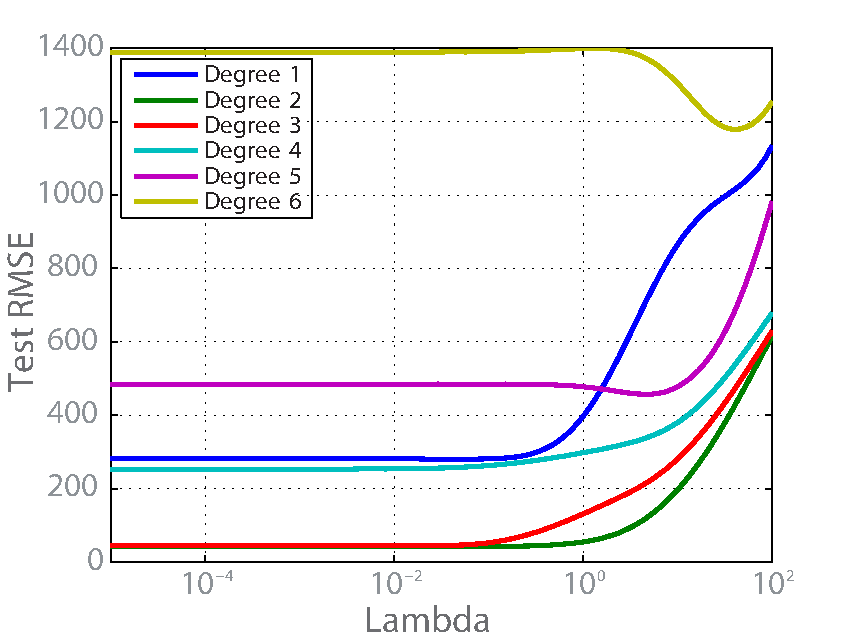
\includegraphics[trim=0mm 0mm 10mm 5mm, clip=true, width=.475\columnwidth]{figures/RegressionRightLambda.pdf}
		\label{fig:RegressionRightLambda}}
	\hfill
	\subfigure[Learning curve for the regression task. After the 80\%-20\% split for train-test data, the test error stabilizes and nears the train error.]
		{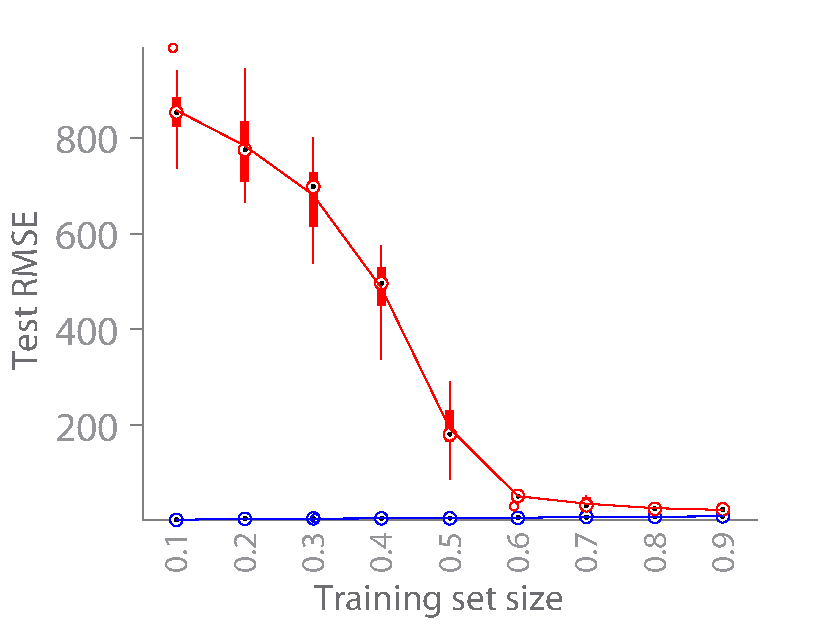
\includegraphics[trim=0mm 0mm 15mm 5mm, clip=true, width=.475\columnwidth]{figures/RegressionLearningCurve2.pdf}
		\label{fig:RegressionLearningCurve}}
	\caption{Comparison of different lambda and degree combinations. Learning curve for regression.}
\end{figure}

%We also investigated the effect of polynomial basis functions on our prediction
%accuracy.

In algorithms 7-9 from Figure \ref{fig:RegressionHist}, we have used
polynomial basis functions with different degrees.
For algorithm 7 we squared all data entrie for both "left" and "right" data splits,
 and in algorithm 8 we used degrees 2 and 3. 
 It can be seen that these feature transformations significantly improve the prediction accuracy 
 compared to the algorithms which did not employ them.

Figure \ref{fig:RegressionRightLambda} shows a plot of the test RMSE for the "right" split, 
for different $\lambda_R$. 
The various curves show the RMSE when the input features have been transformed by raising 
them to the corresponding degree. 
From the figure it can be seen that degree 2 and 3 clearly outperform all other degrees. 
A similar conclusion can be drawn by observing algorithms 7 and 8 from Figure \ref{fig:RegressionHist}. 
In addition, from Figure \ref{fig:RegressionRightLambda} it can be seen that all degrees have 
their optimal lambda value close to 0.

In algorithm 9 we have allowed the features of the "left" and the "right" splits to be transformed with i
ndependent basis function. The optimal degree for the "left" split is 2, and for the "right" split is 3. 
The assembly of steps contained in algorithm 9 constitutes our final model, 
which we will use for providing predictions for the values in $\mathbf{X}_{te}$.


\subsubsection{Learning curve}

To finalize the discussion for regression, we show a plot of the learning curve in 
Figure \ref{fig:RegressionLearningCurve}. 
The plot is produced by using our final algorithm 9, while changing the ratio of train and test data.
At the beginning the train RMSE is close to 0, since the training data is very limited, 
and the model is overfitting, hence the huge test error. 
As the amount of training data increases, we observe that the test error rapidly decreases, 
nears the train error and stabilizes after 80\%-20\%. 
This tells us that the amount of training data is sufficient for the calibration of our algorithm 9.

%We tried several feature transformations. We found that we get a small improvement in performance when we take $\sqrt{|X_{ni}|}$ for all entries of $\mathbf{X}$. We did not check (due to lack of time) whether it matters if we apply this to one variable or all. We performed experiments similar to the last section (although one should really do cross-validation). Values of lambda were kept same as the last section. 

%We compare three methods. First is a baseline where we do not use any input variables i.e. mean value of the output. The second method is the ridge regression described in previous section. The third method is ridge regression with a feature transformation. The first method gave RMSE of around 3 which was way worse than the other two methods.

%The RMSE for the last two methods are shown in Fig. \ref{fig:summary}. We see that both test and train error decrease, however it appears that the improvement is very little and may not be significant.

\section{Classification}

Classification categorizes the input variables(s) in discrete output classes or categories. It is used for predicting the categories for new (unobserved) data samples. For this task, we will train linear binary classifiers which we will later use to classify unseen (test) input variables.

\subsection{Data Description}

The data format for classification is similar to the data which we have already seen for the regression task. We will use the same notation for this task too. The training data for classification consists of $N_{tr}=1500$ input and output data samples. Each input sample is a vector $\mathbf{x}_n$ of dimensionality $D=32$, and all input samples are stored in the matrix $\mathbf{X}_{tr}$. The output variables are binary, since there are two classes, and they are stored in the vector $\mathbf{y}_{tr}$. Each input vector $\mathbf{x}_n$ contains 30 real valued variables and 2 categorical variables. From the categorical variables, 1 has three categories (variable 22), and the other one has four categories (variable 1).

The test dataset consists of $N_{te}=1500$ samples. Here we again observe only the matrix of input variables $\mathbf{X}_{te}$, and we do not have access to the vector of output variables $\mathbf{y}_{te}$. The objective of the classification task is to train a classification model by using the training data, and then to produce class predictions for the unknown output variables $\mathbf{y}_{te}$, corresponding to the input variables in $\mathbf{X}_{te}$. An approximation of the total misclassification error for our model is also expected in the form of RMSE, 0-1 loss and log loss.

\subsection{Data visualization, feature transformations and cleaning}

\begin{figure}[t!]
	\center
	% trim option's parameter order: left bottom right top
	\subfigure[Histogram of the 5th feature for classification in its original space.]
		{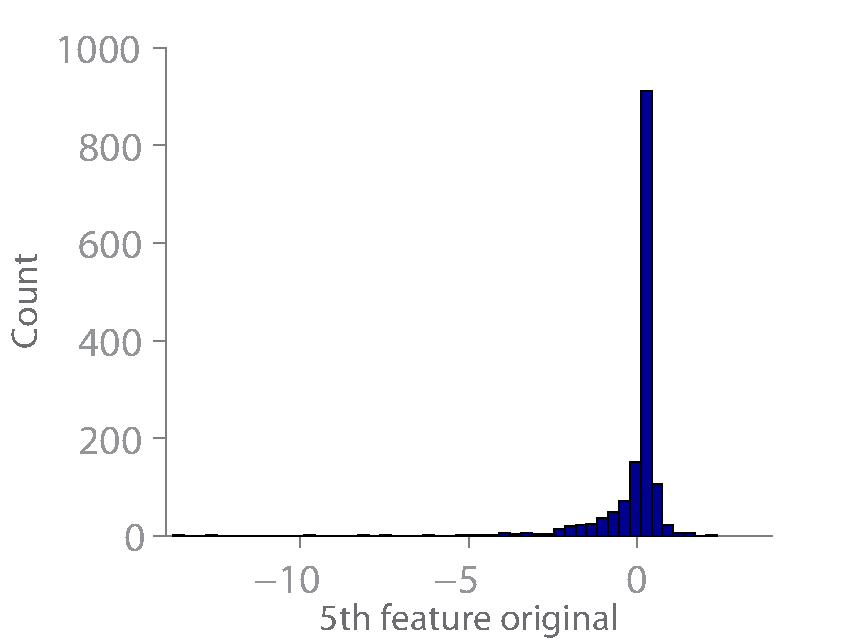
\includegraphics[trim=0mm 0mm 15mm 5mm, clip=true, width=.475\columnwidth]{figures/ClassificationFeature5.pdf}
		\label{fig:ClassificationFeature5}}
	\hfill
	\subfigure[Histogram of the 5th feature for classification in the transformed space.]
		{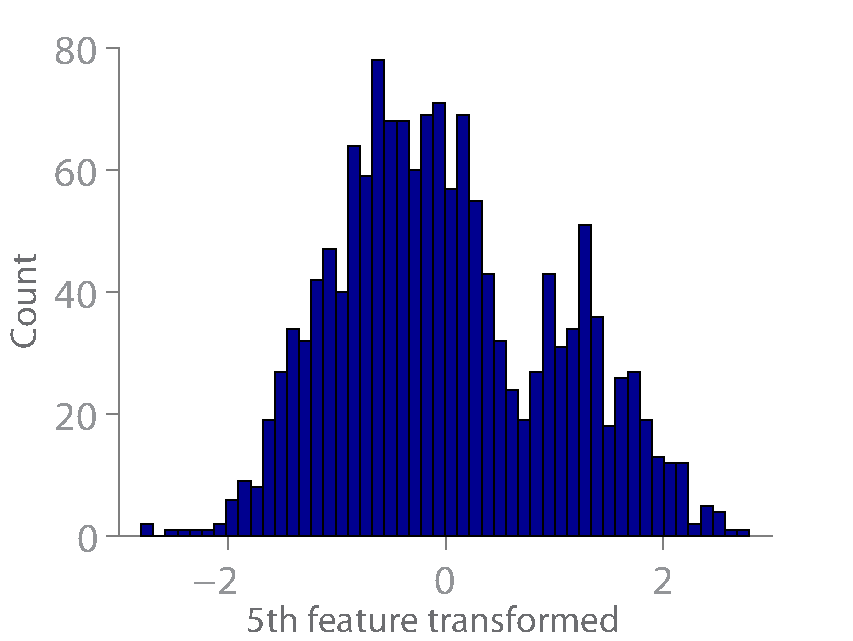
\includegraphics[trim=0mm 0mm 15mm 5mm, clip=true, width=.475\columnwidth]{figures/ClassificationFeature5Transformed.pdf}
		\label{fig:ClassificationFeature5Transformed}}
	\caption{Feature transformations for classification.}
\end{figure}

By plotting the histogram of each continuous input variable, we have noticed that most of them have a Poisson-like distribution of their values. In order to bring their distributions closer to Gaussian, we have applied a feature transformation to each continuous element of the input training matrix $\mathbf{X}_{tr}$, by raising them to the power of $\frac{1}{4}$. Since some of the features had negative entries, we handled them by computing $-\sqrt[4]{-x}$. Figure \ref{fig:ClassificationFeature5} shows the original distribution of the 5th feature. On Figure \ref{fig:ClassificationFeature5Transformed} we can see the Gaussian nature of the distribution of the 5th feature after applying the transformation.

Similarly to the regression task, we again normalize the continuous variables and remove the outliers. We have used the transformed feature space for the removal of the outliers. We eliminated the data vectors which had at least one feature outside of the 4$\sigma$ interval from the mean of the Gaussian of the corresponding feature.

\subsection{Methodology}

\begin{figure}[t!]
	\center
	% trim option's parameter order: left bottom right top
	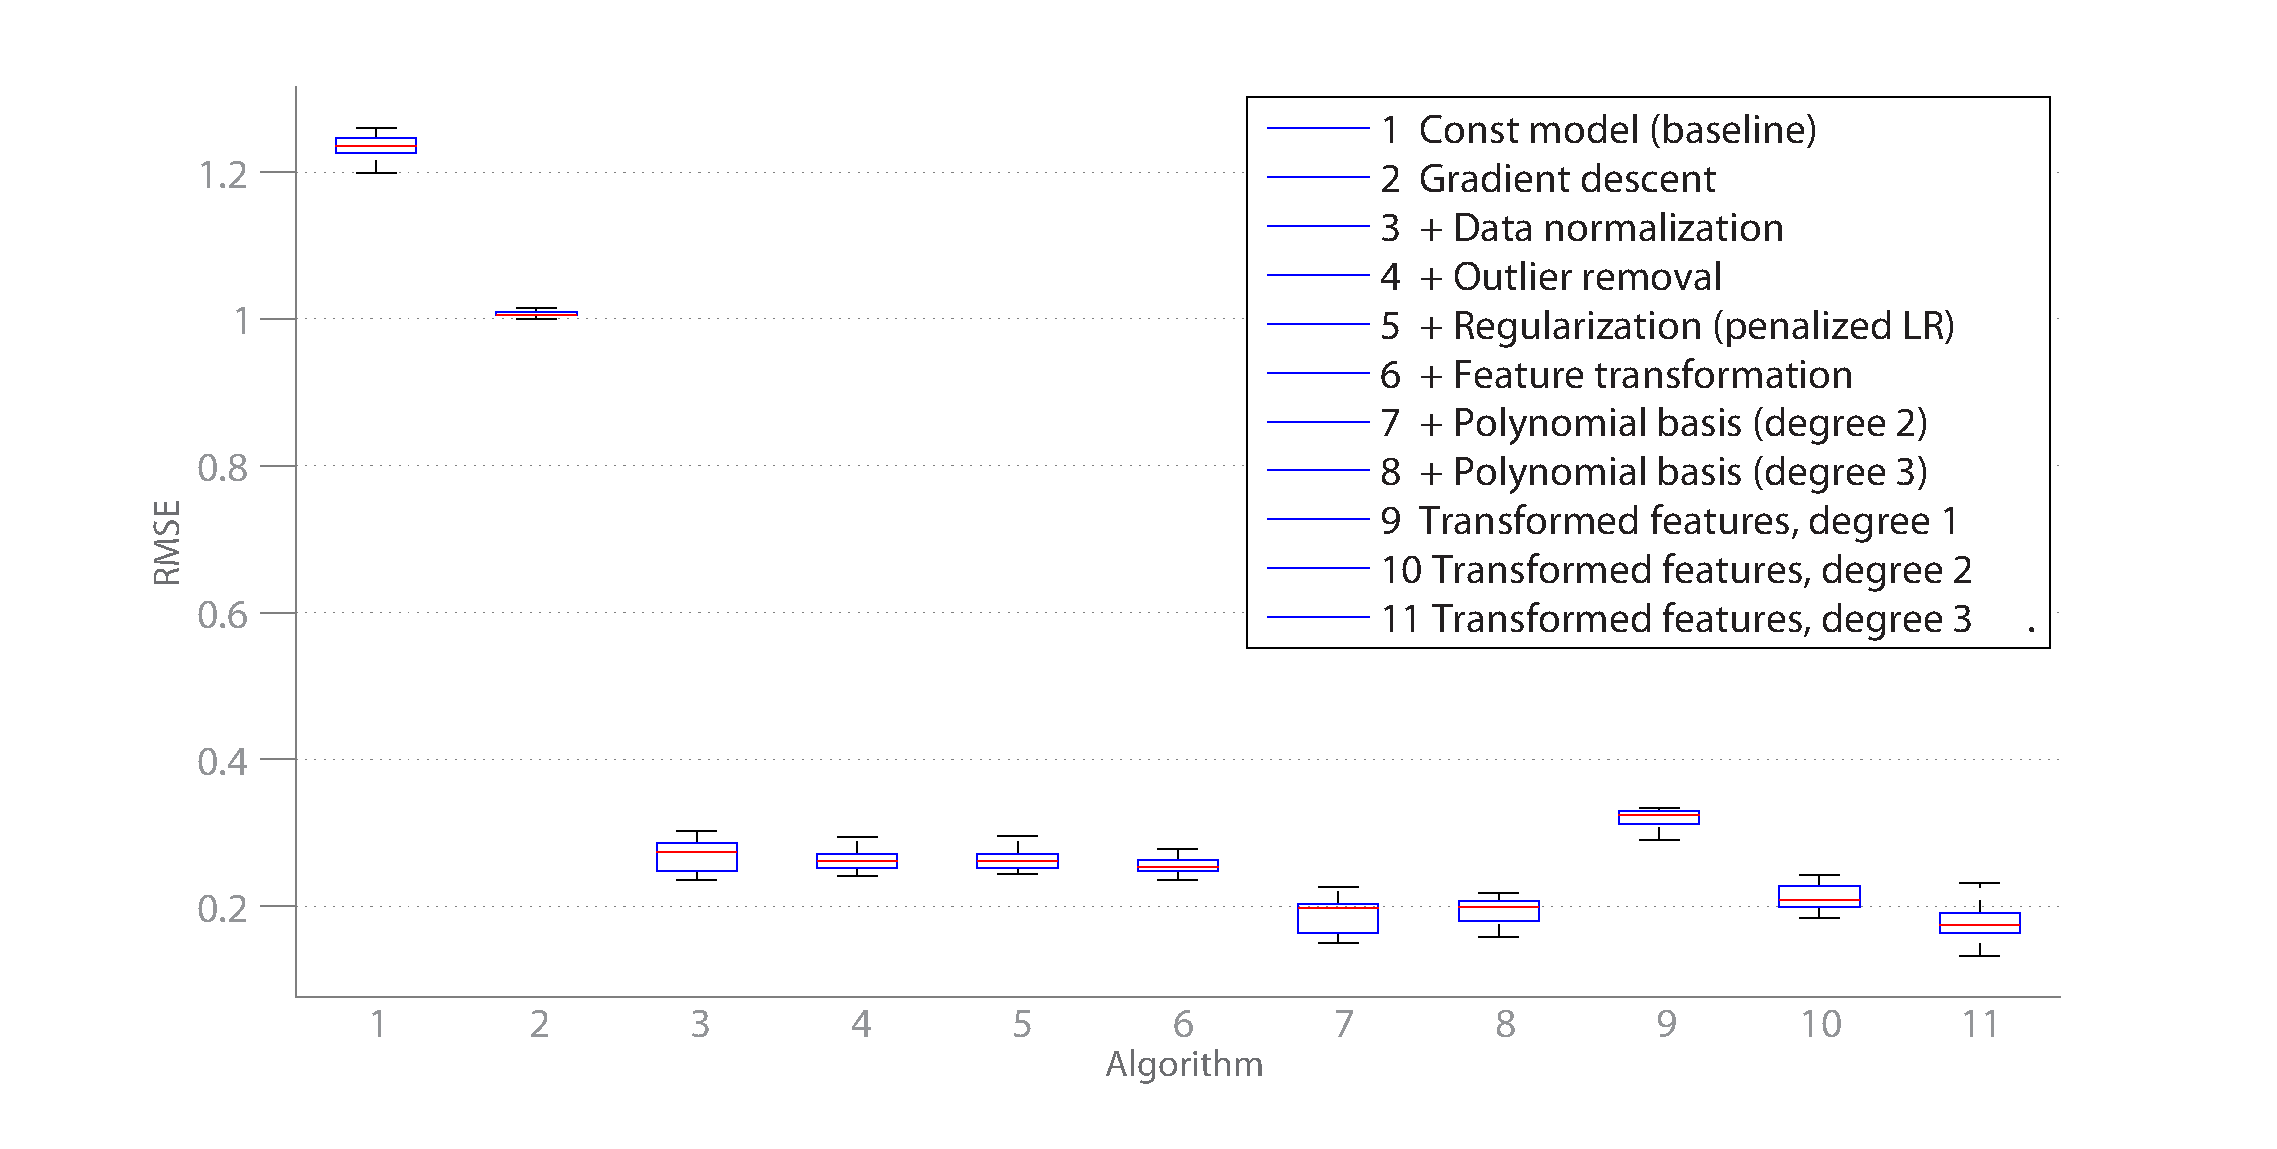
\includegraphics[trim=25mm 10mm 35mm 15mm, clip=true, width=1\columnwidth]{figures/ClassificationHist2.pdf}
	\caption{The box plots show an overview of the mean and standard deviation of the different classification methods and feature transformations which we have tried. Our model of choice is \#11. THIS FIGURE NEED TO BE UPDATED: RMSE > 1}
	\label{fig:ClassificationHist}
\end{figure}

The evaluation of the classification algorithms was done similarly to the evaluation of the regression algorithms. The train-test split was again 80\%-20\%, we have used 10 fold cross validation for determining the necessary method specific parameters, and the mean and variance of the test error was established from 10 trials of randomly permuted train and test datasets.

A comparison of the performance of the various methods which we have used for classification can be seen on Figure \ref{fig:ClassificationHist}. We have used three different linear classification methods, namely: constant model (baseline), logistic regression with gradient descent, and penalized logistic regression. The baseline, as for the regression task does not depend on the input variables; it is just the mean of the output variables, which is passed through the logistic function. The plain logistic regression from algorithm 2 clearly outperforms the baseline. The normalization of the features plays a very important role in lowering the test RMSE in the case of classification, as it can be seen from algorithm 3, which was not the case for regression.

The next interesting algorithm is the addition of the polynomial basis functions in algorithm 7. There, we add non-linear basis function to the original features, by raising them to the power of 2, and in algorithm 8 we also add the basis functions of degree 3. The error decreases slightly, thus the blessing of high dimensionality overweights of curse of dimensionality (we work in 189 dimensional space). It is also important to note that the optimal lambda for the penalized logistic regression (algorithm 5) was calculated from the range $\lambda=$[10$^{-2}$, 10$^{2}$], with 10 samples in between.%, and the optimal value is $\lambda=$?. %It can be noted that even for the ordinary logistic regression we had to use penalized logistic regression with $\lambda=10^{-8}$, since ???. 

In algorithms 9-11, we use only the transformed features, which we have described in the previous subsection, and do not use the original features. The test error for degree 1 is higher then for the original features with degree 1, however, for degrees 2 and 3, the transformed features outperform the original features. The mean test error for algorithm 11 is the lowest across all algorithms, and it uses only a single set of 63 transformed features (and cubed for the non-linear basis). Therefore, it is our model of choice for making the class predictions of the test data stored in $\mathbf{X}_{te}$.

The learning curve for the classification task (not shown due to lack of space) is similar to the learning curve for the regression task, which is shown in Figure \ref{fig:RegressionLearningCurve}. However, there is also a significant difference between the two. Namely, the test error for the classification task continues to decrease, and the training error continues to increase as we reach the 90\%-10\% train-test data split. This suggests that a larger dataset for classification will be useful for our algorithm of choice \#11.

\section{Summary}

In this work we have analysed a regression problem. First, we split the dataset in "left" and "right" data splits, since the data was produced by two sources. Then we tested a set of linear regression algorithms together with different feature transformations, and have settled for ridge regression working with different polynomial basis for the two data splits. The achieved test RMSE is $\approx15$, which outperforms the baseline by 50 fold, and simple least squares by 30 fold.

We also analysed a classification dataset. There we noticed strongly skewed Poisson-like distributions of the input features. Therefore, we transformed the features to assume more Gaussian-like distributions. The model of choice was penalized logistic regression which worked solely on the transformed features, and polynomial basis functions of degree 3. The achieved test RMSE is $\approx0.18$. This model significantly outperformed the baseline and plain logistic regression.

%In this report, we analyzed a regression dataset and found that ridge regression is a reasonable fit. We estimate that the average test error is 1.213 ($\pm$ 0.02). We tried some feature transformation and found that there is a small improvement giving us a test error of around 1.198 ($\pm$ 0.015). This improvement, however, is not significant.

\subsubsection*{Acknowledgments}

The code for the essential functions was developed by all team members independently for error checking and correction. The bulk of the testing was done by Igor and Andrii. Igor produced the final "test errors" and "predictions". Andrii produced the figures, and Marjan summarized our finding by writing most of the report. All team members were engaged in the frequent project discussions.

%We would like to thank Timur for making the dataset for this study, Carlos and Ilija to help conduct the experiments, and all the students who attended the session making it exciting for us. All the code, as well as this report, was written by Emti.

%\subsubsection*{References}

\end{document}